\documentclass[11pt]{article}
\usepackage{setspace}   
\usepackage{titling}
\usepackage{siunitx}    %units in maths
\usepackage[colorlinks=true,linkcolor=black]{hyperref}  %have a review of this
\usepackage{graphicx}
\usepackage{parskip}    %spaced paragraphs
\usepackage{csquotes}   %babel wanted it
\usepackage{graphicx}
\usepackage{pgfgantt}


\usepackage{tabularx}
\usepackage{multirow}
\usepackage{pdflscape}  %pdf support for landscape
\usepackage{adjustbox}  %table sizing

\usepackage[british]{babel} %reduce hyphenation
\renewcommand\britishhyphenmins{60} 

\usepackage{geometry}   %set margins
\geometry{a4paper, margin=2.5cm}

\usepackage{fontspec}
\setmainfont[
    Mapping=tex-text,
    BoldFont={HelveticaNowText-Regular},
    ItalicFont={HelveticaNowText-LightItalic},
    BoldItalicFont={HelveticaNowText-RegIta}
]{[HelveticaNowText-Light]}

\usepackage{biblatex}   %bibliography
\addbibresource{refs.bib}

\usepackage{enumitem}   %reduce list spacing
\setlist{nosep} 

\usepackage{titlesec}   %reduce heading spacing
\titlespacing\section{0pt}{12pt plus 4pt minus 2pt}{0pt plus 2pt minus 2pt}
\titlespacing\subsection{0pt}{12pt plus 4pt minus 2pt}{0pt plus 2pt minus 2pt}
\titlespacing\subsubsection{0pt}{12pt plus 4pt minus 2pt}{0pt plus 2pt minus 2pt}

\setlength{\droptitle}{-4em}     % Eliminate the default vertical space
\addtolength{\droptitle}{-4em}   % Only a guess. Use this for adjustment

\title{\huge Project Feasibility Study\\\Large Portable LoRa Radio Tracker\vspace{0.4em}\\\large 1922268\vspace{-2em}}
% \title{\huge Project Feasibility Study\\\Large Portable LoRa Radio Tracker\\\large}

\preauthor{}
\postauthor{}
\author{}
\predate{}
\date{}
\postdate{}

\begin{document}

\maketitle

\section{Definition}
\subsection{Introduction}
This document is the feasibility study for a LoRa radio based cat tracker.
This project began as a means to provide anxious cat owners peace of mind as to where their pet may be roaming.
Additionally, it will allow pet owners to allow free-roaming where they otherwise would not be able to (i.e. they live in an apartment and cannot install a catflap).
Finally, the intended small form-factor and large tracking range make this product potentially applicable in many other situations besides the one it is designed to cater for.

\subsection{Aim}
This project will attempt to develop a solution to remotely monitoring a moving,
independent target within a 1km radius of a stationary `base'.
It focuses on cats in particular, however is likely applicable to any ranged moving target.
\subsection{Objectives}
This project will be achieved via the following objectives:
\begin{itemize}
    \item 
\end{itemize}

\begin{itemize}
    \item 
    \item 
    \item find appropriate hardware
    \item develop software
    \item manufacture
    \begin{itemize}
        \item transmitter - pcb, casing, mounting
        \item receiver
    \end{itemize}
\end{itemize}

\subsection{Specification List}
\begin{itemize}
    \item Portable
    \begin{itemize}
        \item Small form factor (50mm $\times$ 70mm $\times$ 10mm)
        \item Lightweight (<40g)
        \item Battery powered with enough capacity for a day of roaming (\textasciitilde8 hours)
    \end{itemize}
    \item Suitable for home/consumer use
    \begin{itemize}
        \item Installable with tools a consumer could reasonably be expected to own
        \item Compliant to regulations for consumer products
    \end{itemize}
    \item Reliable
    \begin{itemize}
        \item Stable - minimal downtime, if any
        \item Resistant to software and hardware failures
        \item Repairable without great inconvenience or requiring specialised tools
    \end{itemize}
    \item Suitable Reporting
    \begin{itemize}
        \item Regular updates - updates every minute or better
        \item Capable of reporting in any range between 5m and 1000m 
        \item Suited for an urban environment
    \end{itemize}
    \item Safe
    \begin{itemize}
        \item Not a fire hazard
        \item Not an electrocution hazard
        \item Will not cause burns
        \item Comfortable to wear
        \item Compliant with health, safety, data protection, and environmental regulations
    \end{itemize}
\end{itemize}

\subsection{Scope}
Some pets have particularly independent spirits, and perhaps no more renowned for free-roaming prowess is the domestic cat.
Cats are also particularly well known for going missing for days, weeks, months, or even years, if they return at all.
This project intends to design and develop a product that allows cats the freedom they instinctively seek, 
while providing their owners up-to-date information of their location if, for any reason, it needs to be known.

To achieve this, the cat needs to be fitted with a tracking transmitter of some sort for the period that they are outdoors.
This tracker will transmit location on a regular basis, and will be weather-proof. 
The transmit location will then be received by a permanent fixture at the owner's home, 
after which it can be processed and made presentable, so the cat can be easily located. 

\subsection{Extensions}
The scope of the project currently covers only transmitting location data.
A logical extension would be to render the data in a user-friendly manner.
For example, current and historical location appearing on a map.
With a history of data analysis can be performed, allowing the creation of graphics like heatmaps from location trends. 
Furthermore, if location data is stored (including currently incoming data), 
this can be presented via a webserver such that a user can roam outside and view current location data 
(provided they have an internet connection).

More hardware can be added to the tracker to facilitate enhanced data collection
(accelerometers, piezoelectric sensors, etc.) to recognise activities like types of movement.
A significant feature many trackers utilise is a 'finding' capability of some sort, where the tracker attached to the cat is made to make a noise or flash so it can be found when the owner is within a short range.
This also helps for where a cat returns without the tracker attached, in order to find it again.

\section{Justification}
The intent of this project is not completely novel. Trackers, in particular for house pets (dogs and cats) and farm cows are commonplace \textbf{find that study on cow trackers}.
The project attempts to introduce a new solution to this existent problem.

Products that achieve similar functionality to the one proposed in this project exist. They can be broken down into two types: \begin{itemize}
    \item LTE based - provides completely remote coverage and is only limited by mobile network range. These often come with an upfront cost followed by a subscription fee.
    \item RF based - only useable within a limited range. These are often smaller and lighter, but often come with more limited functionality. 
\end{itemize}
The product of this project falls into the latter category, however it benefits from a greatly enhanced range.
LoRa radio is capable of reliably transmitting over 3km, even in dense suburban areas\cite{augustin:lora}.
In comparison, the Tabcat V2 quotes a range of 152m\cite{tabcat:tracker}. 
While that may be suitable for many owned cats, 
this does not cover the maximum range an owned cat may roam (278m\cite{hammer:urbanisaton}),
or the typical range of a feral cat (1253m\cite{horn:range}).
Furthermore, a single base will be capable of receiving multiple signals.

This product also does not bear reliance on LTE networks, and therefore is suitable to use in regions where infrastucture is lacking.
Furthermore, these types of solutions send and store data to a private server, raising concerns with security and data protection (i.e. an individual's house can be identified from collected location data).

Another style of product uses privately managed networks, built from users of the product (Apple Air Tags, Tile, etc).
This suffers from the same infrastructure problem, except perhaps to a greater degree due to the reliance on distributed consumer use of the product to create the network.

The product to be developed here provides a novel solution

lit review

\section{Design Overview}

o\subsection{Hardware}
two ways to approach

build off a board with bootloader and components - larger form factor

buy a chip and attempt to flash new firmware. advantage of being solderable

\subsection{Software}
arduino ide 

random text


\begin{landscape}
\section{Health \& Safety}
\subsection{Risk Management}
% % \begin{table}[ht]
\centering
\begin{adjustbox}{width=1.8\textwidth,center=\textwidth} 
\begin{tabular}{ |c|c|c|c|c|c|c|c|c| }
\hline
\multicolumn{9}{|c|}{\large\textbf{Risk Register}} \\
\hline
\textbf{Category} & \textbf{Risk Factors} & \textbf{Likelihood (out of 10)} & \textbf{Severity (out of 10)} & \textbf{Total Quantifier} & \textbf{Risk Indicators and time-frame} & \textbf{Response} & \textbf{Status} & \textbf{Actions}\\
\hline
\multirow{3}{*}{\textbf{Resource/Financial}} 
& Budget changes            & a & b & s= a * b & . & . & . & . \\ \cline{2-9}
& Overspending              & a & b & s= a * b & . & . & . & . \\ \cline{2-9}
& Unable to source hardware & a & b & s= a * b & . & . & . & . \\ \cline{2-9}
\hline
\multirow{6}{*}{\textbf{Legal/Contractual}}
& Damage            & a & b & s= a * b & . & . & . & . \\ \cline{2-9}
& Health \& Safety  & a & b & s= a * b & . & . & . & . \\ \cline{2-9}
& Disputes          & a & b & s= a * b & . & . & . & . \\ \cline{2-9}
& Comms             & a & b & s= a * b & . & . & . & . \\ \cline{2-9}
& Disclosure        & a & b & s= a * b & . & . & . & . \\ \cline{2-9}
& IP                & a & b & s= a * b & . & . & . & . \\ \cline{2-9}
\hline
\multirow{3}{*}{\textbf{Time}}
& Delays        & a & b & s= a * b & . & . & . & . \\ \cline{2-9}
& Commitment    & a & b & s= a * b & . & . & . & . \\ \cline{2-9}
& Data loss     & a & b & s= a * b & . & . & . & . \\ \cline{2-9}
\hline
\multirow{2}{*}{\textbf{Method}}
& Equipment issues              & a & b & s= a * b & . & . & . & . \\ \cline{2-9}
& Manufacturing difficulties    & a & b & s= a * b & . & . & . & . \\ \cline{2-9}
\hline
\end{tabular}
\end{adjustbox}
\end{landscape}


\section{Ethics}
some random text

\section{ OLD Definition}
\subsection{Objectives old}
\label{sec:objectives}
This project aims to develop a product that meets the following requirements:


\subsection{Scope old}
While suitable for any remote, moving target, this project will primarly focus on felines and their behaviour. 
The product will be designed to monitor the type range, time, and roaming habits of cats specifically. 

The project itself will explore the design in particular and manufacturing process of the product.

The \nameref{sec:objectives} section outlines the criteria the design will prioritise. 

\subsection{Justification old}

\section{Constraints}
\subsection{General Risks}

\subsection{Time Management}
% 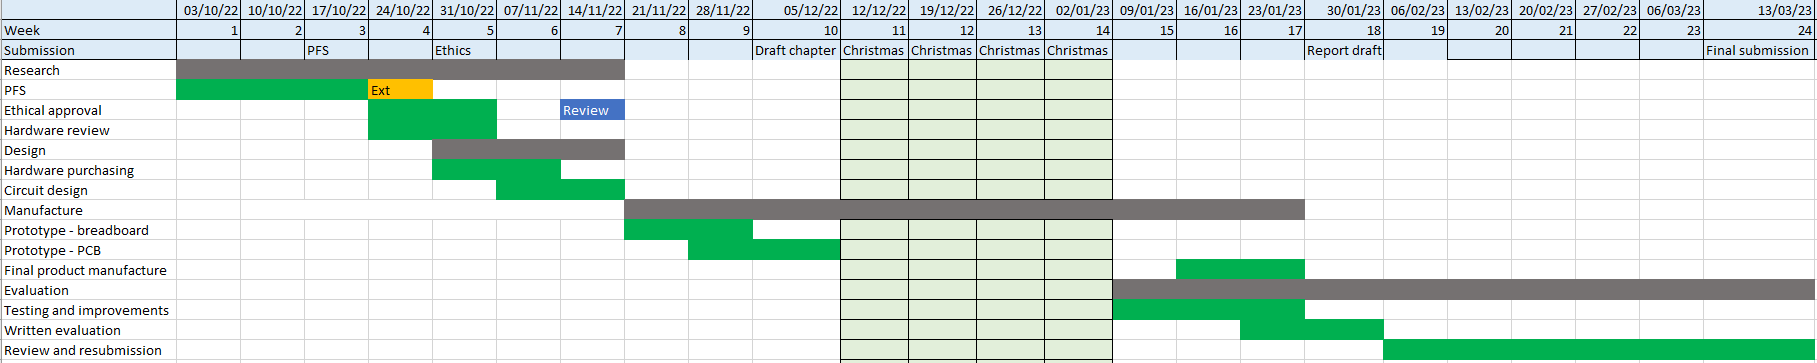
\includegraphics[scale=0.5]{./gantt.png}
\begin{ganttchart}{1}{24}
    \gantttitle{Term 1}{10}\gantttitle{Christmas}{4}\gantttitle{Term 2}{10} \\
    \gantttitlelist{1,...,24}{1} \\
    \ganttgroup{Research}{1}{7} \\
    \ganttbar{PFS}{1}{3} \ganttbar[inline]{E}{4}{4} \\
    \ganttbar{Ethical approval}{4}{5}  \ganttbar[inline]{R}{7}{7}  \\
    \ganttmilestone{Ethics submission}{4} \\
    \ganttbar{Hardware review}{4}{5} \\
    
    \ganttgroup{Design}{5}{7} \\
    \ganttbar{Hardware purchasing}{5}{6} \\
    \ganttbar{Circuit design}{6}{7} \\

    \ganttgroup{Manufacture}{8}{17} \\
    \ganttbar{Prototype - breadboard}{8}{9} \\
    \ganttbar{Prototype - PCB}{9}{10} \\
    
    \ganttmilestone{Draft chapter}{10} \\

    \ganttbar{Final manufacture}{16}{17} \\
    \ganttmilestone{Report draft}{19} \\

    \ganttgroup{Evaluation}{15}{24} \\
    \ganttbar{Test and improvements}{15}{17} \\
    \ganttbar{Written evaluation}{17}{18} \\
    \ganttbar{Review}{19}{24} \\
    \ganttmilestone{Final submission}{23}

    \ganttlink{elem2}{elem3}
    \ganttlink{elem3}{elem4}
\end{ganttchart}
    

\subsection{Security}
gdpr?

\subsection{Intellectual Property}
sufficiently differentiated from existing products?
do i need to check patents?
protecting my IP
\subsection{Sustainability}
Repair
disposal

\subsection{Health and Safety}
animal safety
gdpr?

\subsection{Standards and Legislation}
safey standards - electrical, fire
radio standards

\section{Plan}
\subsection{hardware}

\subsection{Time Management}
there is no time management. only chaos.
\section{Ethics}
\subsection{animal ethics}
\subsection{human ethics}

\section{Evaluation}
what criteria am i am evaluating against 

\printbibliography
\end{document}
